\documentclass[]{article}
\usepackage{lmodern}
\usepackage{amssymb,amsmath}
\usepackage{ifxetex,ifluatex}
\usepackage{fixltx2e} % provides \textsubscript
\ifnum 0\ifxetex 1\fi\ifluatex 1\fi=0 % if pdftex
  \usepackage[T1]{fontenc}
  \usepackage[utf8]{inputenc}
\else % if luatex or xelatex
  \ifxetex
    \usepackage{mathspec}
  \else
    \usepackage{fontspec}
  \fi
  \defaultfontfeatures{Ligatures=TeX,Scale=MatchLowercase}
\fi
% use upquote if available, for straight quotes in verbatim environments
\IfFileExists{upquote.sty}{\usepackage{upquote}}{}
% use microtype if available
\IfFileExists{microtype.sty}{%
\usepackage{microtype}
\UseMicrotypeSet[protrusion]{basicmath} % disable protrusion for tt fonts
}{}
\usepackage[margin=1in]{geometry}
\usepackage{hyperref}
\hypersetup{unicode=true,
            pdftitle={Oxygen Intake Rates - a Measure of Aerobic Fitness},
            pdfauthor={180029941},
            pdfborder={0 0 0},
            breaklinks=true}
\urlstyle{same}  % don't use monospace font for urls
\usepackage{color}
\usepackage{fancyvrb}
\newcommand{\VerbBar}{|}
\newcommand{\VERB}{\Verb[commandchars=\\\{\}]}
\DefineVerbatimEnvironment{Highlighting}{Verbatim}{commandchars=\\\{\}}
% Add ',fontsize=\small' for more characters per line
\usepackage{framed}
\definecolor{shadecolor}{RGB}{248,248,248}
\newenvironment{Shaded}{\begin{snugshade}}{\end{snugshade}}
\newcommand{\KeywordTok}[1]{\textcolor[rgb]{0.13,0.29,0.53}{\textbf{#1}}}
\newcommand{\DataTypeTok}[1]{\textcolor[rgb]{0.13,0.29,0.53}{#1}}
\newcommand{\DecValTok}[1]{\textcolor[rgb]{0.00,0.00,0.81}{#1}}
\newcommand{\BaseNTok}[1]{\textcolor[rgb]{0.00,0.00,0.81}{#1}}
\newcommand{\FloatTok}[1]{\textcolor[rgb]{0.00,0.00,0.81}{#1}}
\newcommand{\ConstantTok}[1]{\textcolor[rgb]{0.00,0.00,0.00}{#1}}
\newcommand{\CharTok}[1]{\textcolor[rgb]{0.31,0.60,0.02}{#1}}
\newcommand{\SpecialCharTok}[1]{\textcolor[rgb]{0.00,0.00,0.00}{#1}}
\newcommand{\StringTok}[1]{\textcolor[rgb]{0.31,0.60,0.02}{#1}}
\newcommand{\VerbatimStringTok}[1]{\textcolor[rgb]{0.31,0.60,0.02}{#1}}
\newcommand{\SpecialStringTok}[1]{\textcolor[rgb]{0.31,0.60,0.02}{#1}}
\newcommand{\ImportTok}[1]{#1}
\newcommand{\CommentTok}[1]{\textcolor[rgb]{0.56,0.35,0.01}{\textit{#1}}}
\newcommand{\DocumentationTok}[1]{\textcolor[rgb]{0.56,0.35,0.01}{\textbf{\textit{#1}}}}
\newcommand{\AnnotationTok}[1]{\textcolor[rgb]{0.56,0.35,0.01}{\textbf{\textit{#1}}}}
\newcommand{\CommentVarTok}[1]{\textcolor[rgb]{0.56,0.35,0.01}{\textbf{\textit{#1}}}}
\newcommand{\OtherTok}[1]{\textcolor[rgb]{0.56,0.35,0.01}{#1}}
\newcommand{\FunctionTok}[1]{\textcolor[rgb]{0.00,0.00,0.00}{#1}}
\newcommand{\VariableTok}[1]{\textcolor[rgb]{0.00,0.00,0.00}{#1}}
\newcommand{\ControlFlowTok}[1]{\textcolor[rgb]{0.13,0.29,0.53}{\textbf{#1}}}
\newcommand{\OperatorTok}[1]{\textcolor[rgb]{0.81,0.36,0.00}{\textbf{#1}}}
\newcommand{\BuiltInTok}[1]{#1}
\newcommand{\ExtensionTok}[1]{#1}
\newcommand{\PreprocessorTok}[1]{\textcolor[rgb]{0.56,0.35,0.01}{\textit{#1}}}
\newcommand{\AttributeTok}[1]{\textcolor[rgb]{0.77,0.63,0.00}{#1}}
\newcommand{\RegionMarkerTok}[1]{#1}
\newcommand{\InformationTok}[1]{\textcolor[rgb]{0.56,0.35,0.01}{\textbf{\textit{#1}}}}
\newcommand{\WarningTok}[1]{\textcolor[rgb]{0.56,0.35,0.01}{\textbf{\textit{#1}}}}
\newcommand{\AlertTok}[1]{\textcolor[rgb]{0.94,0.16,0.16}{#1}}
\newcommand{\ErrorTok}[1]{\textcolor[rgb]{0.64,0.00,0.00}{\textbf{#1}}}
\newcommand{\NormalTok}[1]{#1}
\usepackage{graphicx,grffile}
\makeatletter
\def\maxwidth{\ifdim\Gin@nat@width>\linewidth\linewidth\else\Gin@nat@width\fi}
\def\maxheight{\ifdim\Gin@nat@height>\textheight\textheight\else\Gin@nat@height\fi}
\makeatother
% Scale images if necessary, so that they will not overflow the page
% margins by default, and it is still possible to overwrite the defaults
% using explicit options in \includegraphics[width, height, ...]{}
\setkeys{Gin}{width=\maxwidth,height=\maxheight,keepaspectratio}
\IfFileExists{parskip.sty}{%
\usepackage{parskip}
}{% else
\setlength{\parindent}{0pt}
\setlength{\parskip}{6pt plus 2pt minus 1pt}
}
\setlength{\emergencystretch}{3em}  % prevent overfull lines
\providecommand{\tightlist}{%
  \setlength{\itemsep}{0pt}\setlength{\parskip}{0pt}}
\setcounter{secnumdepth}{0}
% Redefines (sub)paragraphs to behave more like sections
\ifx\paragraph\undefined\else
\let\oldparagraph\paragraph
\renewcommand{\paragraph}[1]{\oldparagraph{#1}\mbox{}}
\fi
\ifx\subparagraph\undefined\else
\let\oldsubparagraph\subparagraph
\renewcommand{\subparagraph}[1]{\oldsubparagraph{#1}\mbox{}}
\fi

%%% Use protect on footnotes to avoid problems with footnotes in titles
\let\rmarkdownfootnote\footnote%
\def\footnote{\protect\rmarkdownfootnote}

%%% Change title format to be more compact
\usepackage{titling}

% Create subtitle command for use in maketitle
\newcommand{\subtitle}[1]{
  \posttitle{
    \begin{center}\large#1\end{center}
    }
}

\setlength{\droptitle}{-2em}

  \title{Oxygen Intake Rates - a Measure of Aerobic Fitness}
    \pretitle{\vspace{\droptitle}\centering\huge}
  \posttitle{\par}
    \author{180029941}
    \preauthor{\centering\large\emph}
  \postauthor{\par}
      \predate{\centering\large\emph}
  \postdate{\par}
    \date{06/11/2018}


\begin{document}
\maketitle

{
\setcounter{tocdepth}{2}
\tableofcontents
}
\pagebreak

\section{Executive Summary}\label{executive-summary}

\pagebreak

\section{Introduction}\label{introduction}

The present report aims to build a model that predicts Oxygen intake
rates (a measure of aerobic fitness) supported on a series of
measurements. The fitness dataset from Rawlings (1998) contains
measurements of the following seven variables obtained from 31 men:

\begin{verbatim}
* Age: Age in years;  
* Weight: Weight in kg;  
* Oxygen: Oxygen intake rate, ml per kg body weight per minute;  
* RunTime: time to run 1.5 miles in minutes;
* RestPulse: heart rate while resting;  
* RunPulse: heart rate at end of run;  
* MaxPulse: maximum heart rate recorded while running; 
\end{verbatim}

From the data set fitness.csv a linear model (predicting Oxygen) will be
developed. The bootstrapping function used to provide confidence
intervals came from an original function provided by Donovan (2018),
which was improved at a later stage.

The report uses R 3.5.1 software (R Core Team, 2018). It was produced a
linear model which was fitted in each analysis and the bootstrap used to
generate confidence intervals for each of the covariates of interest. We
aim to exclude variables that present, essentially, the same information
about response avoiding this way collinearity.

The reasonability of the assumptions on which the model is based were
assessed:

\begin{verbatim}
1. Linearity  
2. Homoscedasticity  
3. Independence  
4. Normality  
\end{verbatim}

Bootstrap methods were used in order draw conclusion to hypothesis tests
in regards to the significance of the relationships between the response
and the parameter estimates. If the confidence interval contains zero,
one fails to reject the null hypothesis, and if it does not contain
zero, one can reject the null hypothesis.

\section{Exploratory Findings}\label{exploratory-findings}

\subsection{Add title}\label{add-title}

Based on our fitness data set, we are going to implement a Linear
Regression Model in which explanatory variables (e.g.~Age, Weight,
RunTime, RestPulse, RunPulse and MaxPulse) will help explain or predict
the behaviour of the response variable (Oxygen). The model is specified
as follows:

..

\begin{verbatim}
## 
## Call:
## lm(formula = Oxygen ~ Age + Weight + RunTime + RestPulse + RunPulse + 
##     MaxPulse, data = fitness)
## 
## Coefficients:
## (Intercept)          Age       Weight      RunTime    RestPulse  
##   102.93448     -0.22697     -0.07418     -2.62865     -0.02153  
##    RunPulse     MaxPulse  
##    -0.36963      0.30322
\end{verbatim}

A first approach to the relatioship between the variables within our
\textbf{fitnessLM} model present the following results:

\begin{figure}
\centering
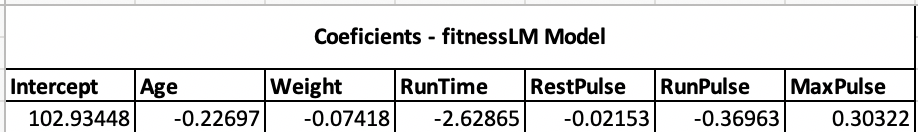
\includegraphics{images/1_fitnessLM_sum.png}
\caption{fitnessLM}
\end{figure}

\begin{itemize}
\item
  (Intercept) = 102.93448. This value represents the value of the
  intercept \(\beta_0\),\\
  when all other \(\beta\) are zero. Therefore, y = \(\beta_0\) = Oxygen
  = 102.93448.
\item
  RunTime = -2.62865. Meaning that everytime RunTime increases by 1
  unit, the Oxygen level decreases by 2.6.
\end{itemize}

In order to forsee how our fitnessLM model is behaving, it can be
produced a \textbf{summary(fitnessLM)} of the model, given the
variables.

\begin{verbatim}
## 
## Call:
## lm(formula = Oxygen ~ Age + Weight + RunTime + RestPulse + RunPulse + 
##     MaxPulse, data = fitness)
## 
## Residuals:
##     Min      1Q  Median      3Q     Max 
## -5.4026 -0.8991  0.0706  1.0496  5.3847 
## 
## Coefficients:
##              Estimate Std. Error t value Pr(>|t|)    
## (Intercept) 102.93448   12.40326   8.299 1.64e-08 ***
## Age          -0.22697    0.09984  -2.273  0.03224 *  
## Weight       -0.07418    0.05459  -1.359  0.18687    
## RunTime      -2.62865    0.38456  -6.835 4.54e-07 ***
## RestPulse    -0.02153    0.06605  -0.326  0.74725    
## RunPulse     -0.36963    0.11985  -3.084  0.00508 ** 
## MaxPulse      0.30322    0.13650   2.221  0.03601 *  
## ---
## Signif. codes:  0 '***' 0.001 '**' 0.01 '*' 0.05 '.' 0.1 ' ' 1
## 
## Residual standard error: 2.317 on 24 degrees of freedom
## Multiple R-squared:  0.8487, Adjusted R-squared:  0.8108 
## F-statistic: 22.43 on 6 and 24 DF,  p-value: 9.715e-09
\end{verbatim}

The \textbf{Residual Standard Error (2.317)} gives us an idea of how far
the Oxygen levels are from the fitted model.

\textbf{Multiple R-Squared = 0.8487}. Almost 85\% of the variation in
Oxygen can be explained by our model.

\textbf{p-value = 9.715e-09}. This value is extremely small, smaller
than 0.05. Therefore, we \textbf{reject the Null Hypothesis (\(\H_0\))}
which assumes that all the model coefficients (\(\beta_0\),
\(\beta_1\),\ldots{},\(\beta_n\)) are zero(0).

\textbf{Pr (\textgreater{}\textbar{}t\textbar{})} gives us the p-value
for the t-test. In this case, all the values which are below 0.05 are of
interest to our model as it can be improved by those. ..

In this particular case, and looking at the value of \textbf{Weight
(0.18687)}, it can be observed that it is greater than 0.05. Therefore,
\textbf{it fails to reject the \(\H_0\)} (Null Hypothes) which is based
on the assumption that all the coefificients (\(\beta_0\),
\(\beta_1\),\ldots{},\(\beta_n\)) are equal to zero. In this scenario,
having to remove a variable from the model, the variable Weight would be
one of the possibilities, for instance.

\subsection{Collinearity}\label{collinearity}

it can be said that, when 2 variables are highly correlated, then there
is collinearity. In fact, at this stage, what we want is to ``exclude
variables that offer essentially the same information about response,
i.e., we want to avoid collinearity.

vif: Calculates variance-inflation and generalized variance-inflation
factors for linear, generalized linear, and other models. In this case
RunPulse (8.437273) and MaxPulse (8.743848) have very similar values,
meaning that they are correlated. Therefore, these variables offer,
essencially, the same information. So, the varible with the highest
value (MaxPulse) can be omitted. display if bigger than 5 they are
correlated therefore give same info and we

\begin{verbatim}
##       Age    Weight   RunTime RestPulse  RunPulse  MaxPulse 
##  1.512836  1.155329  1.590868  1.415589  8.437274  8.743848
\end{verbatim}

\begin{verbatim}
##       Age    Weight   RunTime RestPulse  RunPulse  MaxPulse 
##     FALSE     FALSE     FALSE     FALSE      TRUE      TRUE
\end{verbatim}

\subsection{The new model less
MaxPlus}\label{the-new-model-less-maxplus}

updated model removed MaxPulse - we now have the new fit for the
original model

\begin{verbatim}
## 
## Call:
## lm(formula = Oxygen ~ Age + Weight + RunTime + RestPulse + RunPulse, 
##     data = fitness)
## 
## Coefficients:
## (Intercept)          Age       Weight      RunTime    RestPulse  
##   116.48761     -0.28528     -0.05184     -2.70392     -0.02711  
##    RunPulse  
##    -0.12628
\end{verbatim}

\subsection{final Model}\label{final-model}

The main objective is to find a balance and have a good set of
covariates within our model. If we look only at a few set of variables
we are likely to be disregarding valuable information. On the other way
around, if we include, in our model, both essential and non-essential
variables in a model, the standard error, confidence interval and,
p-values tend to be larger. (g17, 2.5.1) In order to determine the
finalModel, it will be used the function step(), which uses the Akaike
Information Criterion (AIC) to select the model,based in the following
rule: the lower the AIC the better the model.

-----using command
step()------------------------------------------------------

\begin{verbatim}
## Start:  AIC=61.96
## Oxygen ~ Age + Weight + RunTime + RestPulse + RunPulse
## 
##             Df Sum of Sq    RSS    AIC
## - RestPulse  1     0.905 156.23 60.139
## - Weight     1     5.011 160.34 60.943
## <none>                   155.33 61.958
## - RunPulse   1    36.204 191.53 66.453
## - Age        1    47.085 202.41 68.166
## - RunTime    1   267.469 422.80 91.000
## 
## Step:  AIC=60.14
## Oxygen ~ Age + Weight + RunTime + RunPulse
## 
##            Df Sum of Sq    RSS    AIC
## - Weight    1      4.60 160.83 59.037
## <none>                  156.23 60.139
## - RunPulse  1     38.88 195.11 65.027
## - Age       1     46.54 202.77 66.221
## - RunTime   1    346.82 503.06 94.388
## 
## Step:  AIC=59.04
## Oxygen ~ Age + RunTime + RunPulse
## 
##            Df Sum of Sq    RSS    AIC
## <none>                  160.83 59.037
## - RunPulse  1     39.89 200.72 63.905
## - Age       1     42.29 203.12 64.274
## - RunTime   1    370.44 531.27 94.080
\end{verbatim}

now i have the final model with RunPulse, Age, RunTime The AIC value is
now (59.04). Removing either RunPulse, or Age, or RunTime would result
in a much higher AIC. Therefore it is better to keep the model as it is.

\section{CHECKING THE MODEL
ASSUMPTIONS}\label{checking-the-model-assumptions}

\section{ASSESSING LINEARITY}\label{assessing-linearity}

conclude about the plot - age and RunPulse are similar and close to
zero. The steeper the slop the better, the covariate RunTime gives us
more info about the selected model so Runtime is the most important
variable within the model.

\section{Appendix}\label{appendix}

\subsubsection{Code}\label{code}

\begin{Shaded}
\begin{Highlighting}[]
\NormalTok{fitnessLM <-}\StringTok{ }\KeywordTok{lm}\NormalTok{(Oxygen }\OperatorTok{~}\StringTok{ }\NormalTok{Age }\OperatorTok{+}\StringTok{ }\NormalTok{Weight }\OperatorTok{+}\StringTok{ }\NormalTok{RunTime }\OperatorTok{+}\StringTok{ }\NormalTok{RestPulse }\OperatorTok{+}\StringTok{ }\NormalTok{RunPulse }\OperatorTok{+}\StringTok{ }\NormalTok{MaxPulse, }
                \DataTypeTok{data =}\NormalTok{ fitness)}

\NormalTok{fitnessLM}
\end{Highlighting}
\end{Shaded}


\end{document}
